\documentclass{beamer}
\usetheme[white]{Wisconsin}
\usepackage{longtable}
\usepackage{listings}
\usepackage{color}
%% The amssymb package provides various useful mathematical symbols
\usepackage{amssymb}
%% The amsthm package provides extended theorem environments
\usepackage{amsthm} \usepackage{amsmath} \usepackage{tmadd,tmath}
\usepackage[mathcal]{euscript} \usepackage{color}
\usepackage{textcomp}
\usepackage{algorithm,algorithmic}
\definecolor{listinggray}{gray}{0.9}
\definecolor{lbcolor}{rgb}{0.9,0.9,0.9}
\lstset{
  backgroundcolor=\color{lbcolor},
  tabsize=4,
  rulecolor=,
  language=c++,
  basicstyle=\scriptsize,
  upquote=true,
  aboveskip={1.5\baselineskip},
  columns=fixed,
  showstringspaces=false,
  extendedchars=true,
  breaklines=true,
  prebreak =
  \raisebox{0ex}[0ex][0ex]{\ensuremath{\hookleftarrow}},
  frame=single,
  showtabs=false,
  showspaces=false,
  showstringspaces=false,
  identifierstyle=\ttfamily,
  keywordstyle=\color[rgb]{0,0,1},
  commentstyle=\color[rgb]{0.133,0.545,0.133},
  stringstyle=\color[rgb]{0.627,0.126,0.941},
}

%% colors
\setbeamercolor{boxheadcolor}{fg=white,bg=UWRed}
\setbeamercolor{boxbodycolor}{fg=black,bg=white}


%%---------------------------------------------------------------------------%%
\author{Stuart R. Slattery
  \\ Engineering Physics Department
  \\ University of Wisconsin - Madison
}

\date{\today} 
\title{Simplified $P_N$ Equations} 
\begin{document}
\maketitle

%%---------------------------------------------------------------------------%%
\begin{frame}{DTK Update}
  \begin{itemize}
  \item M \& C paper accepted - recommended for journal
  \item Corresponding with MOOSE team lead at INL
    \begin{itemize}
    \item Happy with DTK performance for Geometry/Mesh code-to-code
      coupling
    \item Building new solver framework around DTK in MOOSE
    \item Includes moving data between hierarchies in hierarchal
      solve system
    \item Details to come - seems to be based on domain
      decomposition methods
    \item Interested in more complex communicator structures
    \item Core DTK functionality should remain unmodified
    \item Higher-level MIMD support required - INL framework
    \end{itemize}
  \end{itemize}
\end{frame}

%%---------------------------------------------------------------------------%%
\begin{frame}{MCLS Update}
  \begin{itemize}
  \item M \& C paper accepted for domain leakage approximations for
    Markov chains
  \item Linear solver abstract numerical algorithm interfaces
    completed and tested
  \item Incorporated into Exnihilo with tests - can now be used as a
    linear solver
  \item Now we have to study the linear system...
  \end{itemize}
\end{frame}

%%---------------------------------------------------------------------------%%
\begin{frame}{Neutron Transport Solution Methods}

  \begin{multline}
    \hat{\Omega} \cdot \vec{\nabla} \psi(\vec{r},\hat{\Omega},E) +
    \sigma(\vec{r},E) \psi(\vec{r},\hat{\Omega},E) = \\ \int \int
    \sigma_s(\vec{r},E' \rightarrow E,\hat{\Omega}' \rightarrow
    \hat{\Omega}) \psi(\vec{r},\hat{\Omega}',E') d\Omega' dE' +
    q(\vec{r},\hat{\Omega},E)
    \label{eq:general_transport}
  \end{multline}

  \begin{itemize}
  \item $S_N$ transport is expensive
    \begin{itemize}
    \item Difficult to parallelize: sweeps in space, pipelining in
      angle, energy decoupling
    \item Large storage requirements
    \item Ray effects
    \end{itemize}
  \item $P_N$ equations still expensive
    \begin{itemize}
    \item Complicated system: $(N+1)^2$ equations in 3D
    \item Coupling of equations through both angular moments and
      spatial derivatives
    \end{itemize}
  \end{itemize}
\end{frame}

%%---------------------------------------------------------------------------%%
\begin{frame}{$SP_N$ Approximation}
  \begin{itemize}
  \item Ad-hoc generalization of planar $P_N$ equations by Gelbard in
    the 1960's
  \item Rigorous formulation through asymptotic and variational
    analysis in 1990's and 2000's
  \item Simpler system $(N+1)/2$ equations in $3D$
  \item Yields elliptic, diffusion-like equations
  \item Applicable when diffusion theory is applicable: reasonable
    flux gradients, full-core transport
  \item Typically does not converge to transport solution as
    $N\rightarrow \infty$
  \item {\bf Can build the full linear operator}
  \item {\bf Parallelism through the linear solver}
  \end{itemize}
\end{frame}

%%---------------------------------------------------------------------------%%
\begin{frame}{Legendre Polynomials}

  \begin{equation}
    P_l(\mu) = \frac{1}{2^l l!}\frac{d^l}{d \mu^l}(\mu^2-1)^l\:.
    \label{eq:general_legendre_poly}
  \end{equation}

  Orthogonality:
  \begin{equation}
    \int_{-1}^{1} P_l(\mu) P_{l'}(\mu) d\mu = \frac{1}{2l+1}\delta_{l l'}\:,
    \label{eq:legendre_orthog}
  \end{equation}

  Recurrence:
  \begin{equation}
    \mu P_l(\mu) = \frac{1}{2l+1}[(l+1)P_{l+1}(\mu) + l P_{l-1}(\mu)]\:,
    \label{eq:legendre_recurrence}
  \end{equation}

  Addition theorem:
  \begin{equation}
    P_l(\hat{\Omega} \cdot \hat{\Omega}') = \frac{1}{2n+1}\sum_{m=-l}^l
    Y_{lm}(\hat{\Omega})Y^*_{lm}(\hat{\Omega}')\:,
    \label{eq:legendre_addition}
  \end{equation}

  Planar addition theorem:
  \begin{equation}
    P_l(\hat{\Omega} \cdot \hat{\Omega}') = P_l(\mu)P_l(\mu')\:.
    \label{eq:legendre_addition_3}
  \end{equation}

\end{frame}

%%---------------------------------------------------------------------------%%
\begin{frame}{$P_N$ Derivation}
  Monoenergetic, planar 1D transport equation:
  \begin{equation}
    \mu \frac{\partial}{\partial x} \psi(x,\mu) + \sigma(x) \psi(x,\mu)
    = \int d\Omega' \sigma_s(x,\hat{\Omega}' \rightarrow \hat{\Omega})
    \psi(\vec{r},\hat{\Omega}') + \frac{q(x)}{4 \pi}\:.
    \label{eq:mono_transport}
  \end{equation}

  Angular discretization:
  \begin{equation}
    \psi(x,\mu) = \sum_{n=0}^\infty (2n+1)P_n(\mu)\phi_n(x)\:,
    \label{eq:flux_expansion}
  \end{equation}
  \begin{equation}
    \sigma_{sm}(x) = \sum_{m=0}^\infty (2m+1)P_m(\mu)\sigma_s(x)\:,
    \label{eq:scattering_expansion}
  \end{equation}

\end{frame}

%%---------------------------------------------------------------------------%%
\begin{frame}{$P_N$ Derivation}
  Insert expansions:
  \begin{multline}
    \frac{\partial}{\partial x}\Big[\sum_{n=0}^\infty (2n+1) \phi_n \mu
      P_n(\mu) \Big] + \sigma \sum_{n=0}^\infty (2n+1) \phi_n P_n(\mu) =
    \\ \int_{-1}^1 \sum_{m=0}^\infty (2m+1) \sigma_{sm} P_m(\mu_0)
    \sum_{n=0}^\infty (2n+1) \phi_n P_n(\mu') d \mu' + q\:,
    \label{eq:pn_deriv_1}
  \end{multline}

  Use legendre polynomial properties to reduce:
  \begin{equation}
    \sum_{n=0}^\infty \frac{\partial}{\partial x} \frac{1}{2n+1} \Big[
      (n+1) \phi_{n+1} + n \phi_{n-1} \Big] + \sum_{n=0}^\infty \sigma
    \phi_n = \sum_{n=0}^\infty \sigma_{sn} \phi_n + q\delta_{n0}\:.
    \label{eq:pn_deriv_18}
  \end{equation}

\end{frame}

%%---------------------------------------------------------------------------%%
\begin{frame}{$P_N$ Derivation}

  \begin{beamerboxesrounded}[upper=boxheadcolor,lower=boxbodycolor,shadow=true]
    {$P_N$ Equations}
    \begin{equation}
      \frac{1}{2n+1} \frac{\partial}{\partial x}\Big[ (n+1) \phi_{n+1} + n
        \phi_{n-1} \Big] + \Sigma_n \phi_n = q\delta_{n0} \:,
      \label{eq:final_pn_equations}
    \end{equation}
    with $\Sigma_n = \sigma-\sigma_{sn}$ and $n = 0,1,\dotsc,N$ and
    closure: $\phi_{N+1} = 0$
  \end{beamerboxesrounded}

  Example:P5 Equations
  {\small
    \begin{subequations}
      \begin{gather}
        \frac{\partial}{\partial x}\phi_{1} + \Sigma_0 \phi_0 = q\:,\\ 
        \frac{1}{3} \frac{\partial}{\partial x}\Big[ 2
          \phi_{2} + \phi_{0} \Big] + \Sigma_1 \phi_1 = 0\:,\\
        \frac{1}{5} \frac{\partial}{\partial x}\Big[ 3 \phi_{3} + 2
          \phi_{1} \Big] + \Sigma_2 \phi_2 = 0 \:,\\
        \frac{1}{7} \frac{\partial}{\partial x}\Big[ 4 \phi_{4} + 3
          \phi_{2} \Big] + \Sigma_3 \phi_3 = 0 \:,\\
        \frac{1}{9} \frac{\partial}{\partial x}\Big[ 5 \phi_{5} + 4
          \phi_{3} \Big] + \Sigma_4 \phi_4 = 0 \:,\\
        \frac{1}{11} \frac{\partial}{\partial x} 5 \phi_{4} + \Sigma_5
        \phi_5 = 0 \:.
      \end{gather}
      \label{eq:p5_equations}
    \end{subequations}
  }

\end{frame}

%%---------------------------------------------------------------------------%%
\begin{frame}{$SP_N$ Approximation}
  Use odd-order moments in even-order equations to eliminate them:
  \begin{equation}
    \phi_n = \frac{1}{\Sigma_n}\Bigg[ q \delta_{no} -
      \frac{\partial}{\partial x}\Big(\frac{n}{2n+1}\phi_{n-1} +
      \frac{n+1}{2n+1} \phi_{n+1} \Big) \Bigg] \ \ \ \ n=1,3,\cdots N\:, 
    \label{eq:odd_moments}
  \end{equation}

  \begin{multline}
    -\frac{\partial}{\partial x}
    \Bigg[\frac{n}{2n+1}\frac{1}{\Sigma_{n-1}} \frac{\partial}{\partial
        x} \Big(\frac{n-1}{2n-1} \phi_{n-2} + \frac{n}{2n-1}\phi_n \Big)
      \\+ \frac{n+1}{2n+1}\frac{1}{\Sigma_{n+1}}
      \frac{\partial}{\partial x} \Big(\frac{n+1}{2n+3}\phi_n +
      \frac{n+2}{2n+3}\phi_{n+2}\Big) \Bigg] \\+ \Sigma_n \phi_n = q
    \delta_{n0}\ \ \ \ \ \ \ \ \ n = 0,2,4,\cdots,N\:.
    \label{eq:reduced_pn}
  \end{multline}

\end{frame}

%%---------------------------------------------------------------------------%%
\begin{frame}{$SP_N$ Approximation}

  \begin{itemize}
  \item Replace spatial derivatives with general multidimensional gradient
    operators:
  \end{itemize}

  \begin{beamerboxesrounded}[upper=boxheadcolor,lower=boxbodycolor,shadow=true]
    {$SP_N$ Equations}
    \begin{multline}
      -\nabla \cdot \Bigg[\frac{n}{2n+1}\frac{1}{\Sigma_{n-1}} \nabla
        \Big(\frac{n-1}{2n-1} \phi_{n-2} + \frac{n}{2n-1}\phi_n \Big)
        \\+ \frac{n+1}{2n+1}\frac{1}{\Sigma_{n+1}} \nabla
        \Big(\frac{n+1}{2n+3}\phi_n + \frac{n+2}{2n+3}\phi_{n+2}\Big)
        \Bigg] \\+ \Sigma_n \phi_n = q \delta_{n0}\ \ \ \ \ \ \ \ \ n
      = 0,2,4,\cdots,N\:,
      \label{eq:spn_equations}
    \end{multline}
  \end{beamerboxesrounded}

\end{frame}

%%---------------------------------------------------------------------------%%
\begin{frame}{$SP_7$ Example}

  \begin{subequations}
    \begin{gather}
      -\nabla \cdot \frac{1}{3 \Sigma_1} \nabla ( \phi_0 + 2\phi_2 ) +
      \Sigma_0 \phi_0 = q \\ 
      -\nabla \cdot \Bigg[ \frac{2}{15 \Sigma_1} \nabla ( \phi_0 + 2\phi_2
        ) + \frac{3}{35 \Sigma_3}\nabla( 3\phi_2 + 4\phi_4)\Bigg] +
      \Sigma_2 \phi_2 = 0\\
      -\nabla \cdot \Bigg[ \frac{4}{63 \Sigma_3} \nabla ( 3\phi_2 +
        4\phi_4 ) + \frac{5}{99 \Sigma_5}\nabla( 5\phi_4 +
        6\phi_6)\Bigg] + \Sigma_4 \phi_4 = 0\\
      -\nabla \cdot \Bigg[ \frac{6}{143 \Sigma_5} \nabla ( 5\phi_4 +
        6\phi_6 ) + \frac{7}{195 \Sigma_7}\nabla(7\phi_6)\Bigg] +
      \Sigma_6 \phi_6 = 0 \:.
    \end{gather}
    \label{eq:sp7_equations}
  \end{subequations}

\end{frame}

%%---------------------------------------------------------------------------%%
\begin{frame}{$SP_7$ Example}

  Change variables:

  \begin{subequations}
    \begin{gather}
      u_1 = \phi_0 + 2\phi_2 \\
      u_2 = 3\phi_2 + 4\phi_4 \\
      u_3 = 5\phi_4 + 6\phi_6 \\
      u_4 = 7\phi_6 \:,
    \end{gather}
    \label{eq:spn7_subs}
  \end{subequations}

  \begin{subequations}
    \begin{gather}
      \phi_0 = u_1 - \frac{2}{3}u_2 + \frac{8}{15}u_3 -
      \frac{16}{35}u_4 \\
      \phi_2 = \frac{1}{3}u_2 - \frac{4}{15}u_3 + \frac{8}{35}u_4\\ 
      \phi_4 = \frac{1}{5}u_3 - \frac{6}{35}u_4\\
      \phi_6 = \frac{1}{7}u_4\:.
    \end{gather}
    \label{eq:spn7_subs_inverse}
  \end{subequations}

\end{frame}

%%---------------------------------------------------------------------------%%
\begin{frame}{$SP_7$ Example}

  \begin{subequations}
    \begin{gather}
      -\nabla \cdot \frac{1}{3 \Sigma_1} \nabla u_1 + \Sigma_0 \Bigg[
        u_1 - \frac{2}{3}u_2 + \frac{8}{15}u_3 - \frac{16}{35}u_4 \Bigg]
      = -q \\
      -\nabla \cdot \Bigg[ \frac{2}{15 \Sigma_1} \nabla u_1 +
        \frac{3}{35 \Sigma_3} \nabla u_2 \Bigg] + \Sigma_2 \Bigg[
        \frac{1}{3}u_2 - \frac{4}{15}u_3 + \frac{8}{35}u_4 \Bigg] = 0 \\
      -\nabla \cdot \Bigg[ \frac{4}{63 \Sigma_3} \nabla u_2 +
        \frac{5}{99 \Sigma_5} \nabla u_3 \Bigg] + \Sigma_4 \Bigg[
        \frac{1}{5}u_3 - \frac{6}{35}u_4 \Bigg] = 0 \\ 
      -\nabla \cdot \Bigg[ \frac{6}{143 \Sigma_5} \nabla u_3 +
        \frac{7}{195 \Sigma_7} \nabla u_4 \Bigg] + \Sigma_6 \Bigg[
        \frac{1}{7}u_4 \Bigg] = 0 \:.
    \end{gather}
    \label{eq:spn7_subs_equations}
  \end{subequations}

\end{frame}

%%---------------------------------------------------------------------------%%
\begin{frame}{$SP_7$ Example}
Rearrange so that we only have 1 divergence operation in each
equation:

\begin{equation}
  -\nabla \cdot D_n \nabla u_n + \sum_{m=1}^4 A_{nm} u_m =
  q_n\ \ \ \ \ \ \ n = 1,2,3,4\:,
  \label{eq:spn_matrix}
\end{equation}

$\mathbf{D}$ the vector of effective diffusion coefficients:
\begin{equation}
  \mathbf{D} = \Bigg( \frac{1}{3\Sigma_1}\ \ \frac{1}{7\Sigma_3}\ \
  \frac{1}{11\Sigma_5}\ \ \frac{1}{15\Sigma_7} \Bigg)^T\:,
  \label{eq:spn7_diffusion_coeffs}
\end{equation}
$\mathbf{q}$ the vector of source terms where the $0^{th}$ moment
source has now been distributed through the system:
\begin{equation}
  \mathbf{q} = (
  q\ \ -\frac{2}{3}q\ \ \frac{8}{15}q\ \ -\frac{16}{35}q )^T\:,
  \label{eq:spn7_source_vector}
\end{equation}

\end{frame}

%%---------------------------------------------------------------------------%%
\begin{frame}{$SP_7$ Example}
  and $\mathbf{A}$ a matrix of angular scattering terms:
  % NOTE: I copied the following matrix directly out of Tom's tech note
  % on the SPn equations which I am effectively following here because I
  % was feeling lazy. I have verified its correctness.
  {\tiny
    \begin{equation}
      \mathbf{A} = 
      \begin{bmatrix}
        (\Sigma_0) &
        (-\frac{2}{3}\Sigma_0) &
        (\frac{8}{15}\Sigma_0) &
        (-\frac{16}{35}\Sigma_0) \\
        %%
        &&&\\
        %%
        (-\frac{2}{3}\Sigma_0) &
        (\frac{4}{15}\Sigma_0 + \frac{1}{3}\Sigma_2) &
        (-\frac{16}{45}\Sigma_0 - \frac{4}{9}\Sigma_2) &
        (\frac{32}{105}\Sigma_0 + \frac{8}{21}\Sigma_2) \\
        %%
        &&&\\
        %%
        (\frac{8}{15}\Sigma_0) &
        (-\frac{16}{45}\Sigma_0 - \frac{4}{9}\Sigma_2) &
        (\frac{64}{225}\Sigma_0 + \frac{16}{45}\Sigma_2 + \frac{9}{25}\Sigma_4) &
        (-\frac{128}{525}\Sigma_0 - \frac{32}{105}\Sigma_2 - \frac{54}{175}\Sigma_4)
        \\ 
        %%
        &&&\\
        %%
        (-\frac{16}{35}\Sigma_0) &
        (\frac{32}{105}\Sigma_0 + \frac{8}{21}\Sigma_2) &
        (-\frac{128}{525}\Sigma_0 - \frac{32}{105}\Sigma_2 - \frac{54}{175}\Sigma_4)
        & 
        (\frac{256}{1225}\Sigma_0 + \frac{64}{245}\Sigma_2 +
        \frac{324}{1225}\Sigma_4 + \frac{13}{49}\Sigma_6)
      \end{bmatrix}\:.
      \label{eq:A_matrix}
    \end{equation}
  }
\end{frame}

%%---------------------------------------------------------------------------%%
\begin{frame}{Multigroup $SP_N$ equations}

  {\small
    Multigroup, planar, 1D transport equation:
    \begin{equation}
      \mu \frac{\partial}{\partial x} \psi^g(x,\mu) + \sigma^g(x)
      \psi^g(x,\mu) = \sum_{g'=0}^{G} \int
      \sigma_s^{gg'}(x,\hat{\Omega}' \rightarrow \hat{\Omega})
      \psi^{g'}(x,\hat{\Omega}') d\Omega' + \frac{q^g(x)}{4 \pi}\:,
      \label{eq:cart_1d_multigroup}
    \end{equation}
  }
  {\small
    Multigroup $P_N$ Equations:
    \begin{equation}
      \frac{1}{2n+1} \frac{\partial}{\partial x}\Big[ (n+1) \phi^g_{n+1}
        + n \phi^g_{n-1} \Big] +
      \sum_{g'}(\sigma^g\delta_{gg'}-\sigma^{gg'}_{sn}) \phi^g_n =
      q\delta_{n0} \:,
      \label{eq:multigroup_pn_equations}
    \end{equation}
  }
  {\small Scattering Matrix:}
  {\tiny
    \begin{equation}
      \mathbf{\Sigma}_n =
      \begin{bmatrix}
        (\sigma^0-\sigma_{sn}^{00}) & -\sigma_{sn}^{01} & \dots &
        -\sigma_{sn}^{0G} \\ &&&\\ -\sigma_{sn}^{10} &
        (\sigma^1-\sigma_{sn}^{11}) & \dots & -\sigma_{sn}^{1G}
        \\ &&&\\ \vdots & \vdots & \ddots & \vdots
        \\ &&&\\ -\sigma_{sn}^{G0} & -\sigma_{sn}^{G1} & \dots &
        (\sigma^G-\sigma_{sn}^{GG})
      \end{bmatrix}\:.
    \end{equation}
  }

\end{frame}

%%---------------------------------------------------------------------------%%
\begin{frame}{Multigroup $SP_N$ equations}
  
  Multigroup $SP_N$ equations:
  \begin{multline}
    -\nabla \cdot \Bigg[\frac{n}{2n+1}\mathbf{\Sigma_{n-1}}^{-1}
      \nabla \Big(\frac{n-1}{2n-1} \mathbf{\Phi_{n-2}} +
      \frac{n}{2n-1}\mathbf{\Phi_n} \Big) \\+
      \frac{n+1}{2n+1}\mathbf{\Sigma_{n+1}}^{-1} \nabla
      \Big(\frac{n+1}{2n+3}\mathbf{\Phi_n} +
      \frac{n+2}{2n+3}\mathbf{\Phi_{n+2}}\Big) \Bigg] \\+
    \mathbf{\Sigma_n} \mathbf{\Phi_n} = \mathbf{q}
    \delta_{n0}\ \ \ \ \ \ \ \ \ n = 0,2,4,\cdots,N\:.
    \label{eq:multigroup_spn_equations}
  \end{multline}

  Change variables and rearrange again:
  \begin{equation}
    -\nabla \cdot \mathbb{D}_n \nabla \mathbb{U}_n + \sum_{m=1}^4
    \mathbb{A}_{nm} \mathbb{U}_m = \mathbb{Q}_n\:,
    \label{eq:spn_multigroup_system}
  \end{equation}

\end{frame}

%%---------------------------------------------------------------------------%%
\begin{frame}{Spatial discretization}

  \begin{itemize}
    \item Equations to this point ignored spatial discretization
    \item All are valid in the domain anywhere (but not necessarily on
      the boundary)
    \item Exnihilo uses a finite volume discretization on a
      rectilinear grid
    \item Discretization is constistent, based on a conservation law
      approach
    \item Flux is balanced in a cell, currents continuous across
      cell/material boundaries
  \end{itemize}

\end{frame}

%%---------------------------------------------------------------------------%%
\begin{frame}{$SP_N$ Numerical Spectral Analysis}

  \begin{itemize}
    \item Monte Carlo methods for have strong restrictions on the
      eigenvalues of the operator for convergence
    \item MCSA has the same restrictions on the outer stationary
      iteration
    \item We need to compute these eigenvalues for various forms of
      the $SP_N$ equations to verify convergence of these methods.
  \end{itemize}

  We need eigenvalues for $\mathbf{A}$, $\mathbf{H_{J}}$, and
  $\mathbf{H_{GS}}$ with:
  \begin{equation}
    \mathbf{H_{J}} = \mathbf{I} - \mathbf{D}^{-1} \mathbf{A}
    \label{eq:jacobi_iteration_matrix}
  \end{equation}
  where $\mathbf{D} = diag(\mathbf{A})$ and 
  \begin{equation}
    \mathbf{H_{GS}} = (\mathbf{L+D})^{-1}\mathbf{U}
    \label{eq:gauss_seidel_iteration_matrix}
  \end{equation}

\end{frame}

%%---------------------------------------------------------------------------%%
\begin{frame}{$SP_7$, $P_3$, 3 groups, reflecting boundaries}

  \begin{columns}

    \begin{column}{0.5\textwidth}
      \begin{figure}[h!]
        \centering
        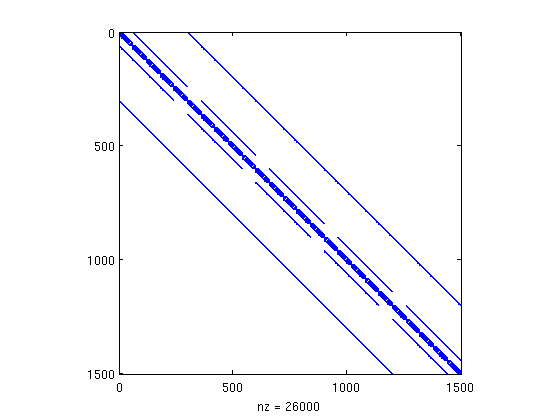
\includegraphics[width=2.5in,clip]{opSpySPn7P3G3.png}
        \caption{\textbf{Linear operator sparsity pattern}}
      \end{figure}
    \end{column}

    \begin{column}{0.5\textwidth}
      \begin{figure}[h!]
        \centering
        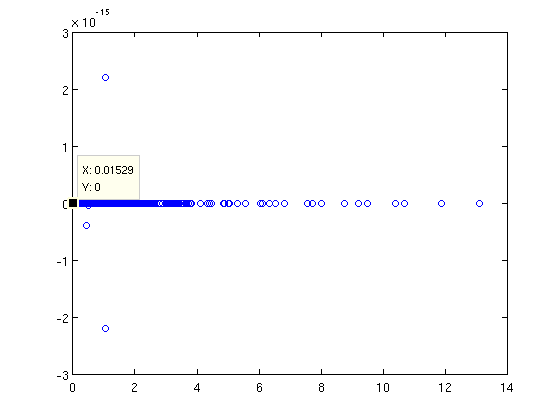
\includegraphics[width=2.5in,clip]{opSPn7P3G3.png}
        \caption{\textbf{Linear operator eigenvalues}}
      \end{figure}
    \end{column}

  \end{columns}

\end{frame}

%%---------------------------------------------------------------------------%%
\begin{frame}{$SP_7$, $P_3$, 3 groups, reflecting boundaries}

  \begin{columns}

    \begin{column}{0.5\textwidth}
      \begin{figure}[h!]
        \centering
        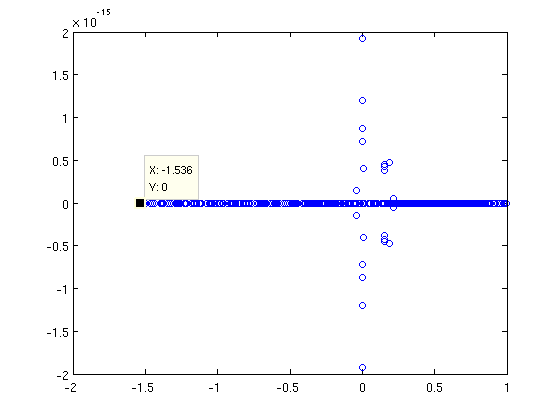
\includegraphics[width=2.5in,clip]{SPn7P3G3.png}
        \caption{\textbf{Jacobi iteration matrix eigenvalues}}
      \end{figure}
    \end{column}

    \begin{column}{0.5\textwidth}
      \begin{figure}[h!]
        \centering
        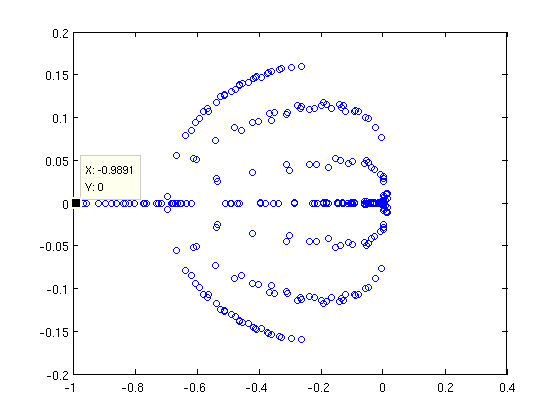
\includegraphics[width=2.5in,clip]{gsSPn7P3G3.png}
        \caption{\textbf{Gauss-Seidel iteration matrix eigenvalues}}
      \end{figure}
    \end{column}

  \end{columns}

\end{frame}

%%---------------------------------------------------------------------------%%

\end{document}
